\documentclass[12pt]{extarticle}

\usepackage[utf8]{inputenc}
\usepackage[T1]{fontenc}
\usepackage{lmodern}
\usepackage{graphicx}
\usepackage{color}
\usepackage{hyperref}
\usepackage{amsmath}
\usepackage{amsfonts}
\usepackage{epstopdf}
\usepackage[table]{xcolor}
\usepackage[a4paper, total={6in, 10in}]{geometry}
\usepackage{enumitem}
\usepackage[export]{adjustbox}
\usepackage{algorithm2e}

\graphicspath{ {./Figures/} }

\begin{document}

{\Large Andrew Sivaprakasam | Warm-Up 2 Write-up}

GitHub Repo: \url{https://github.com/sivaprakasaman/Numerical_Methods_BME/} 

\section{Solving a Nonlinear Single Equation}
\stepcounter{subsection}


\subsection{Bisection Method Thought Exercise | Task List 1-A}

\begin{enumerate}
\item A, B, and C demonstrate cases where there may or may not be a root between $f(x_1)$ and $f(x_m)$ when their product is greater than zero. 
**\textbf{Note:} when I drew these, I accidentally put $x_u$ instead of $x_m$
\item A and B also demonstrate that there may be multiple roots between $x_1$ and $x_u$ when their product is greater than zero.
\\
\begin{center}
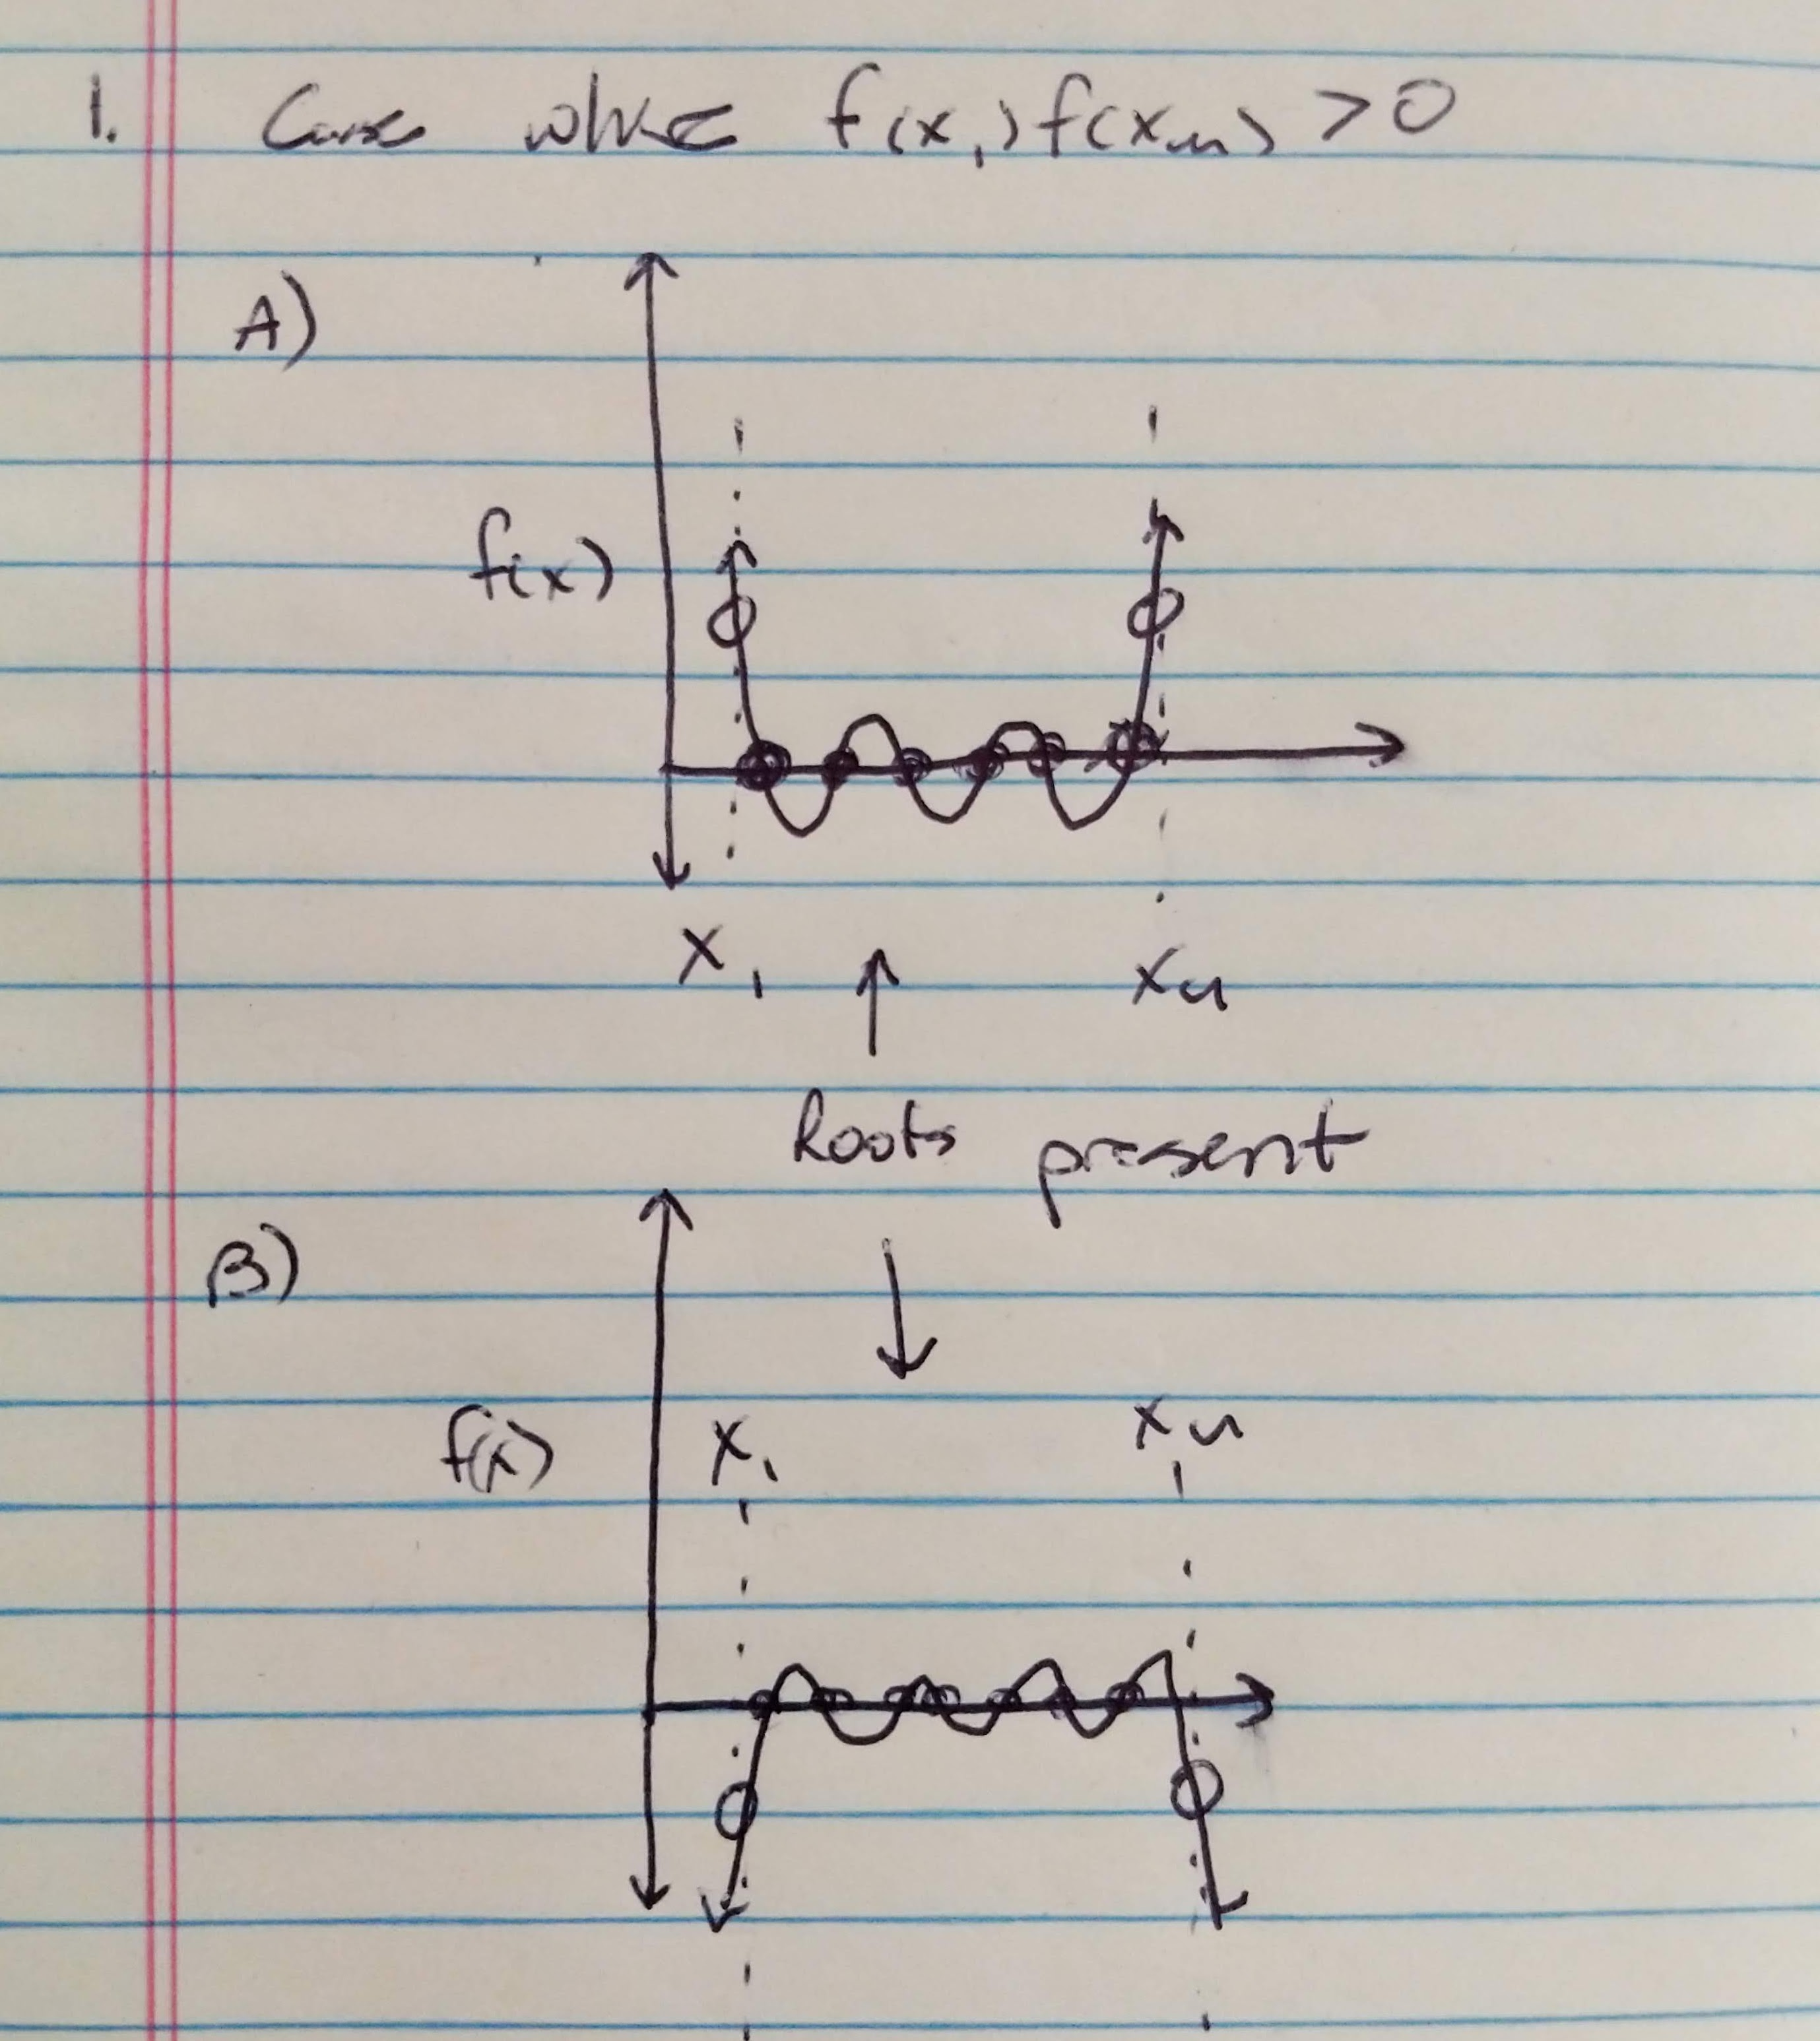
\includegraphics[width = .45\textwidth]{pic_1}
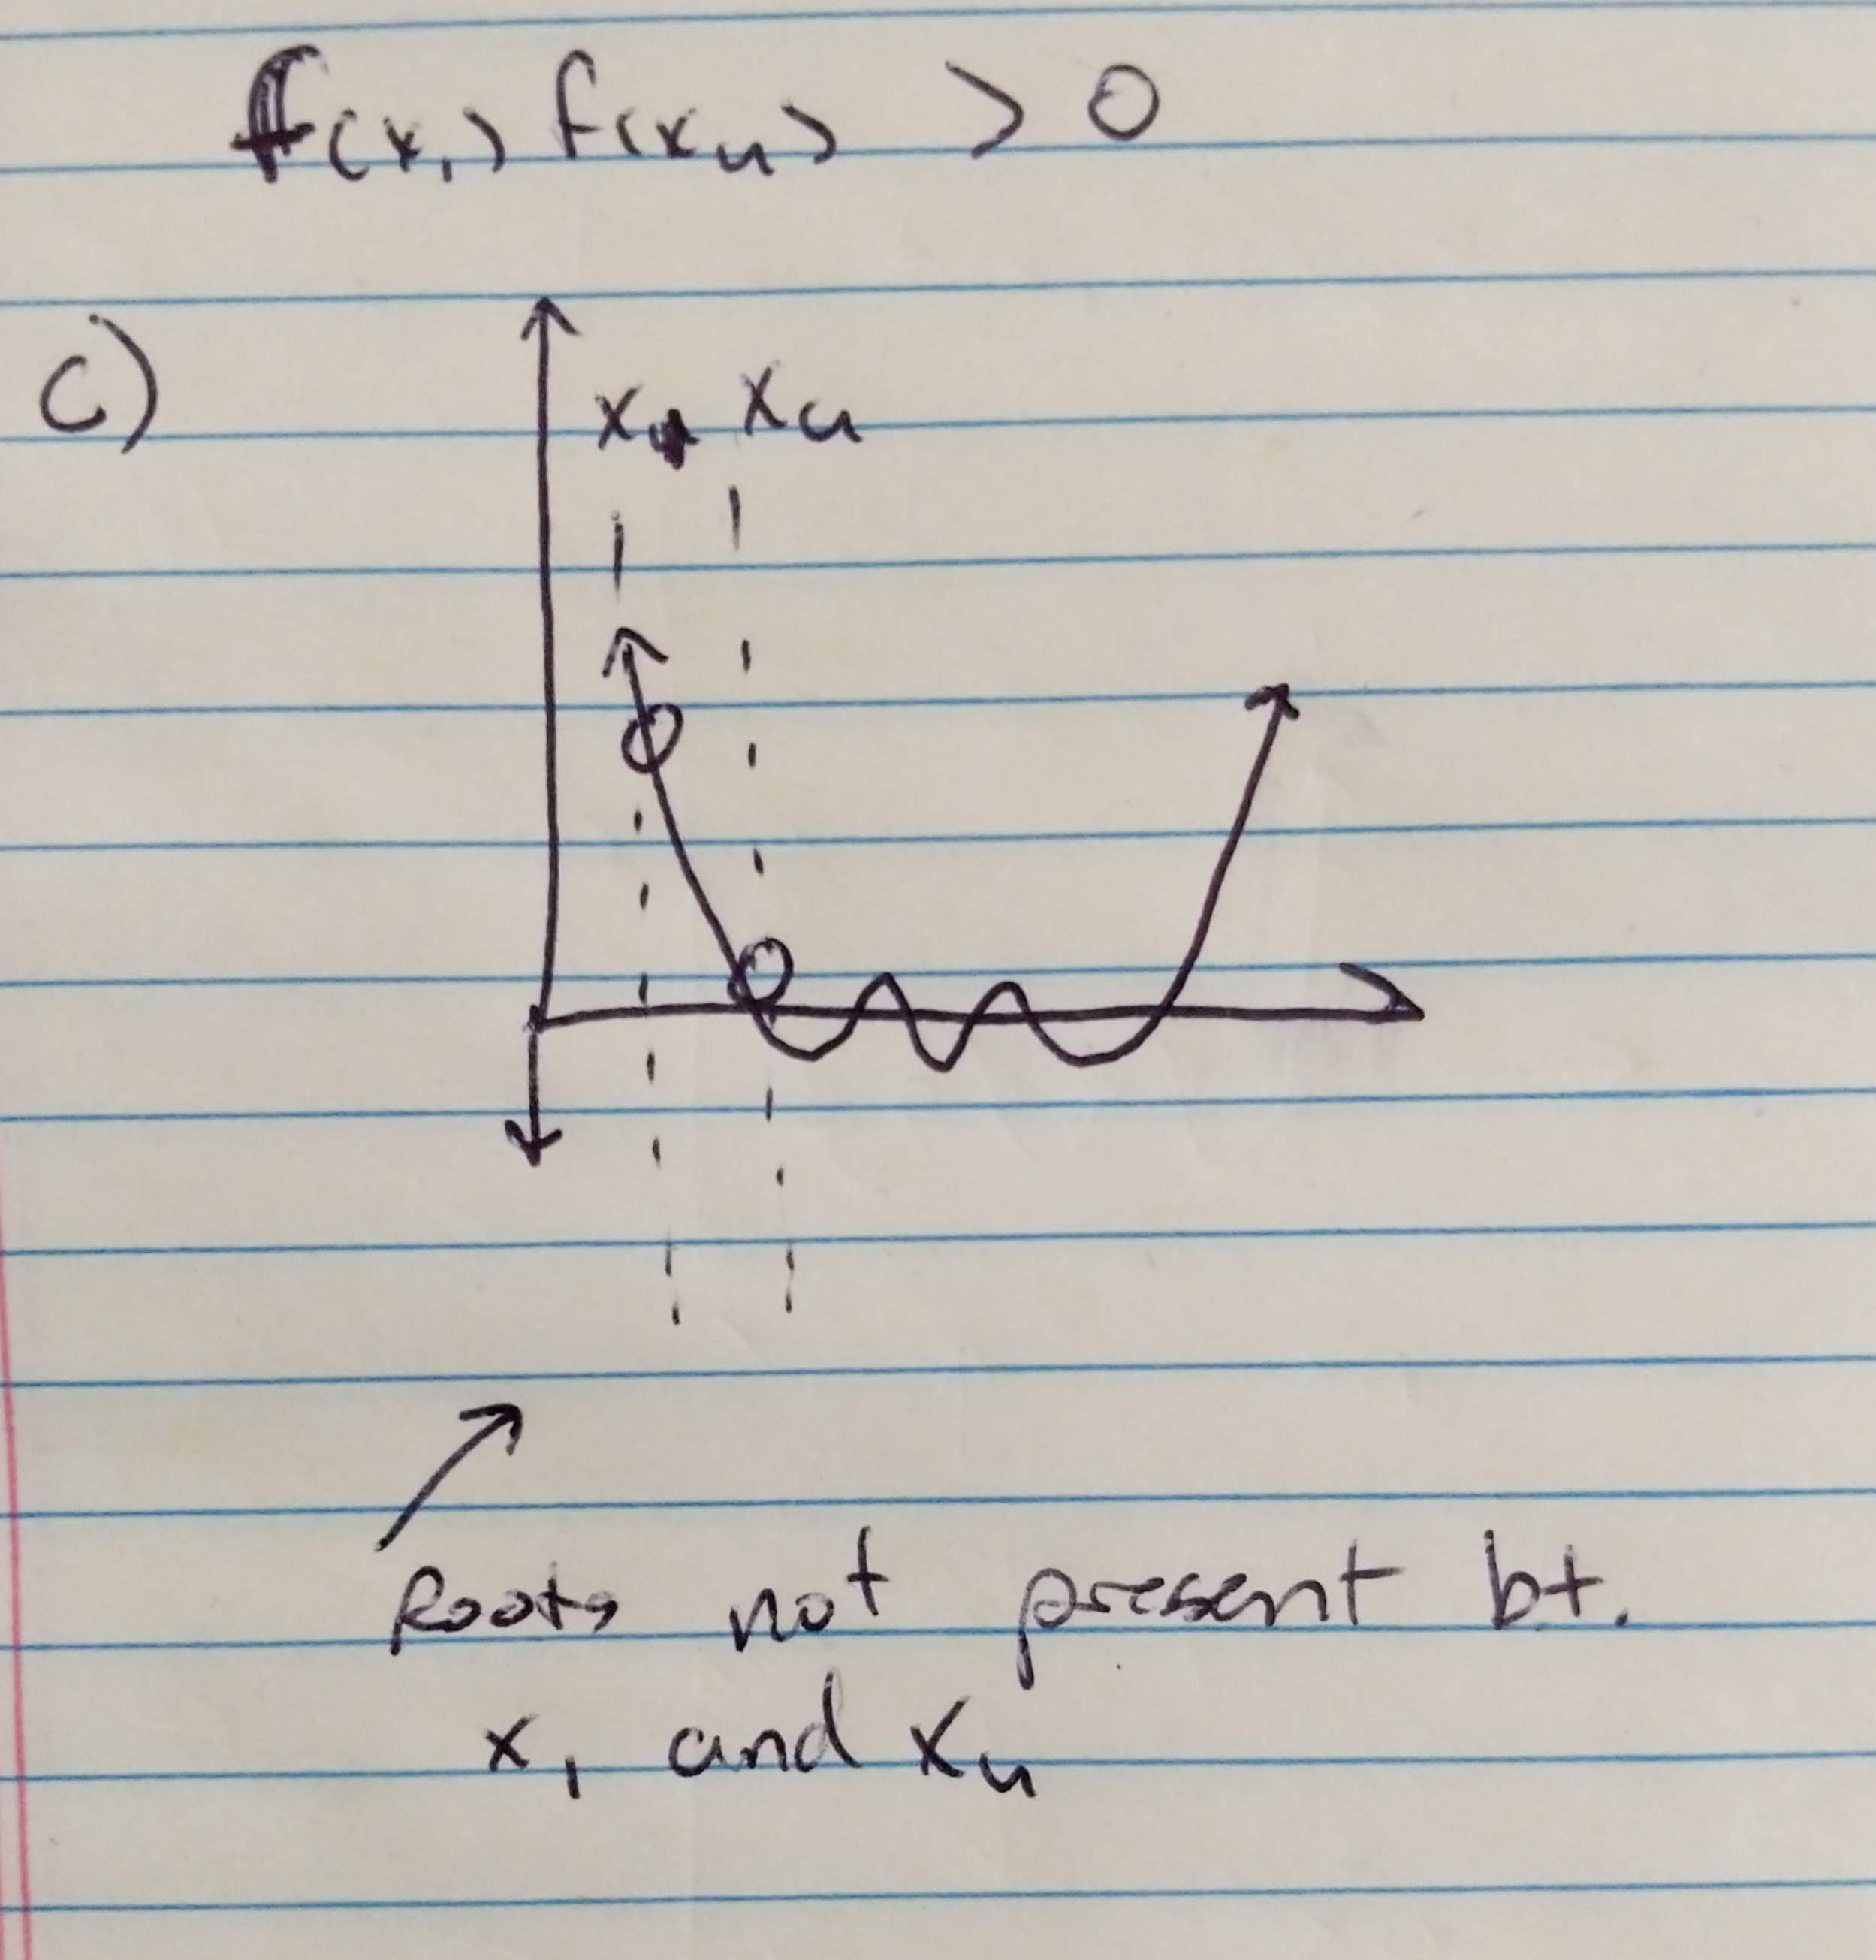
\includegraphics[width = .45\textwidth]{pic_2}
\end{center}

\item Bisection Method Flowchart:
\begin{center}
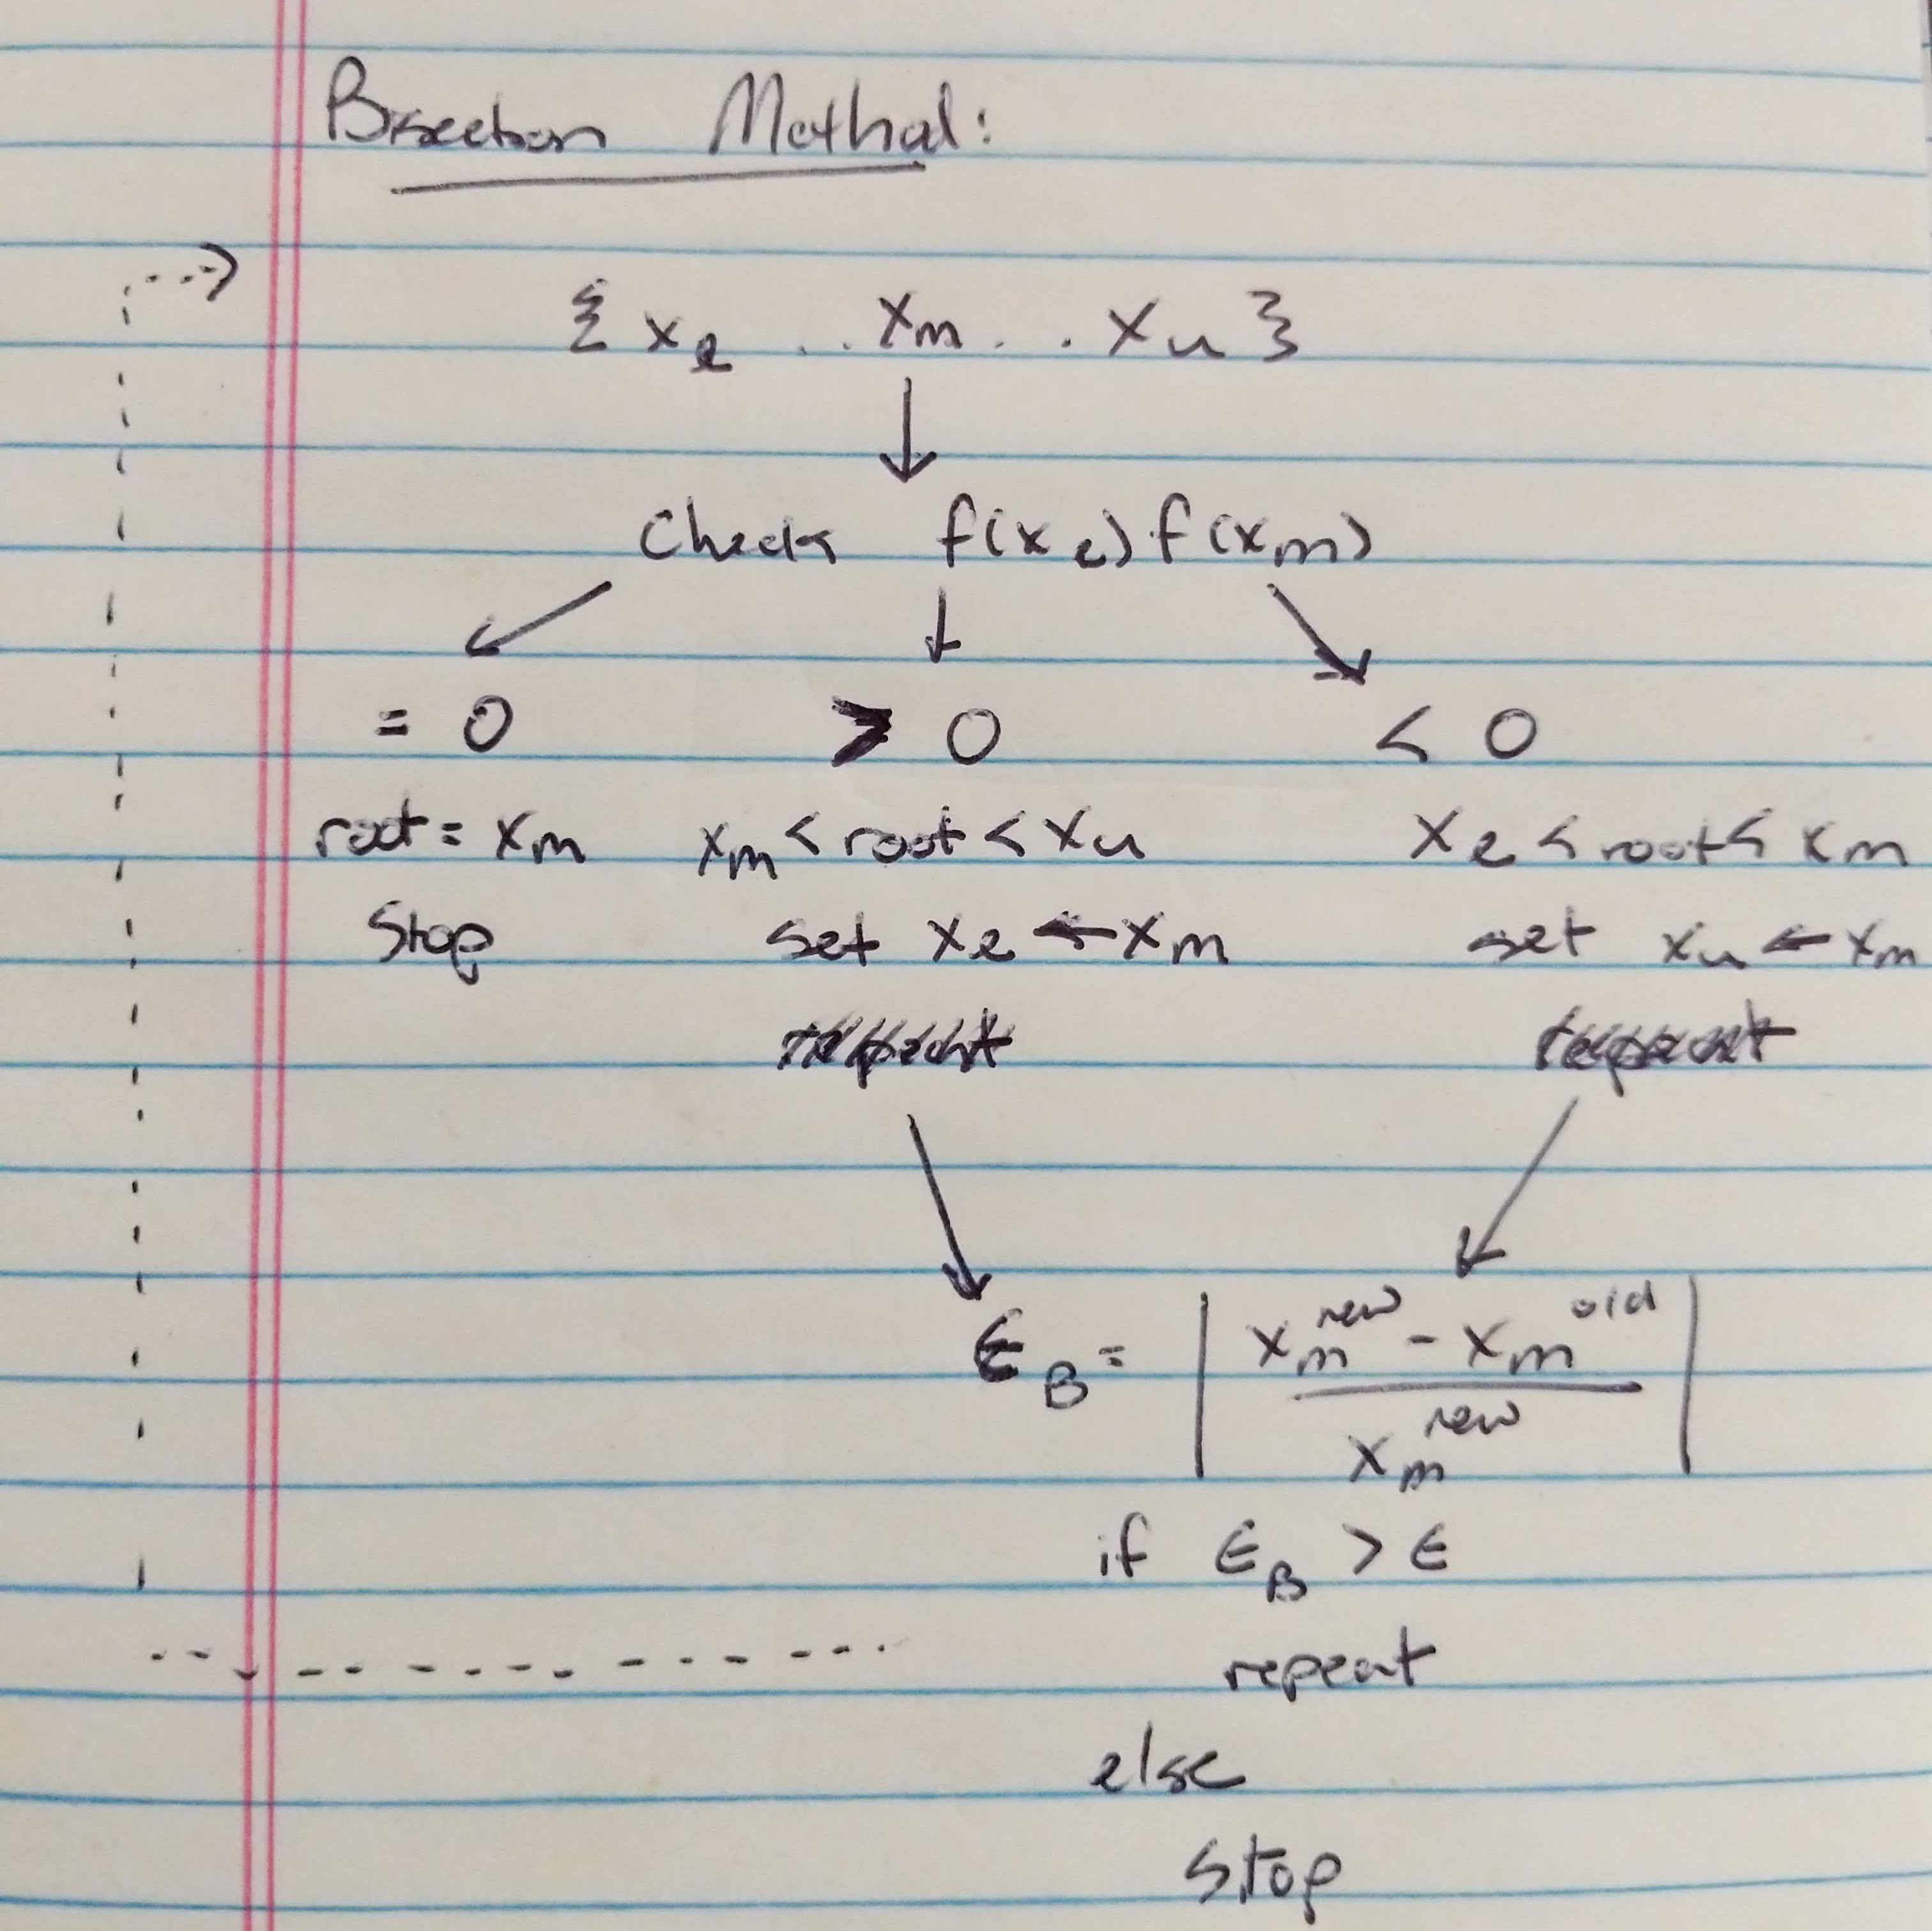
\includegraphics[width = .6\textwidth]{pic_3}
\end{center}
\end{enumerate}

\newpage
\subsection{Newton's Method | Task List 1-B}
\begin{enumerate}
\item Below is a flowchart demonstrating Newton's Method:
\begin{center}
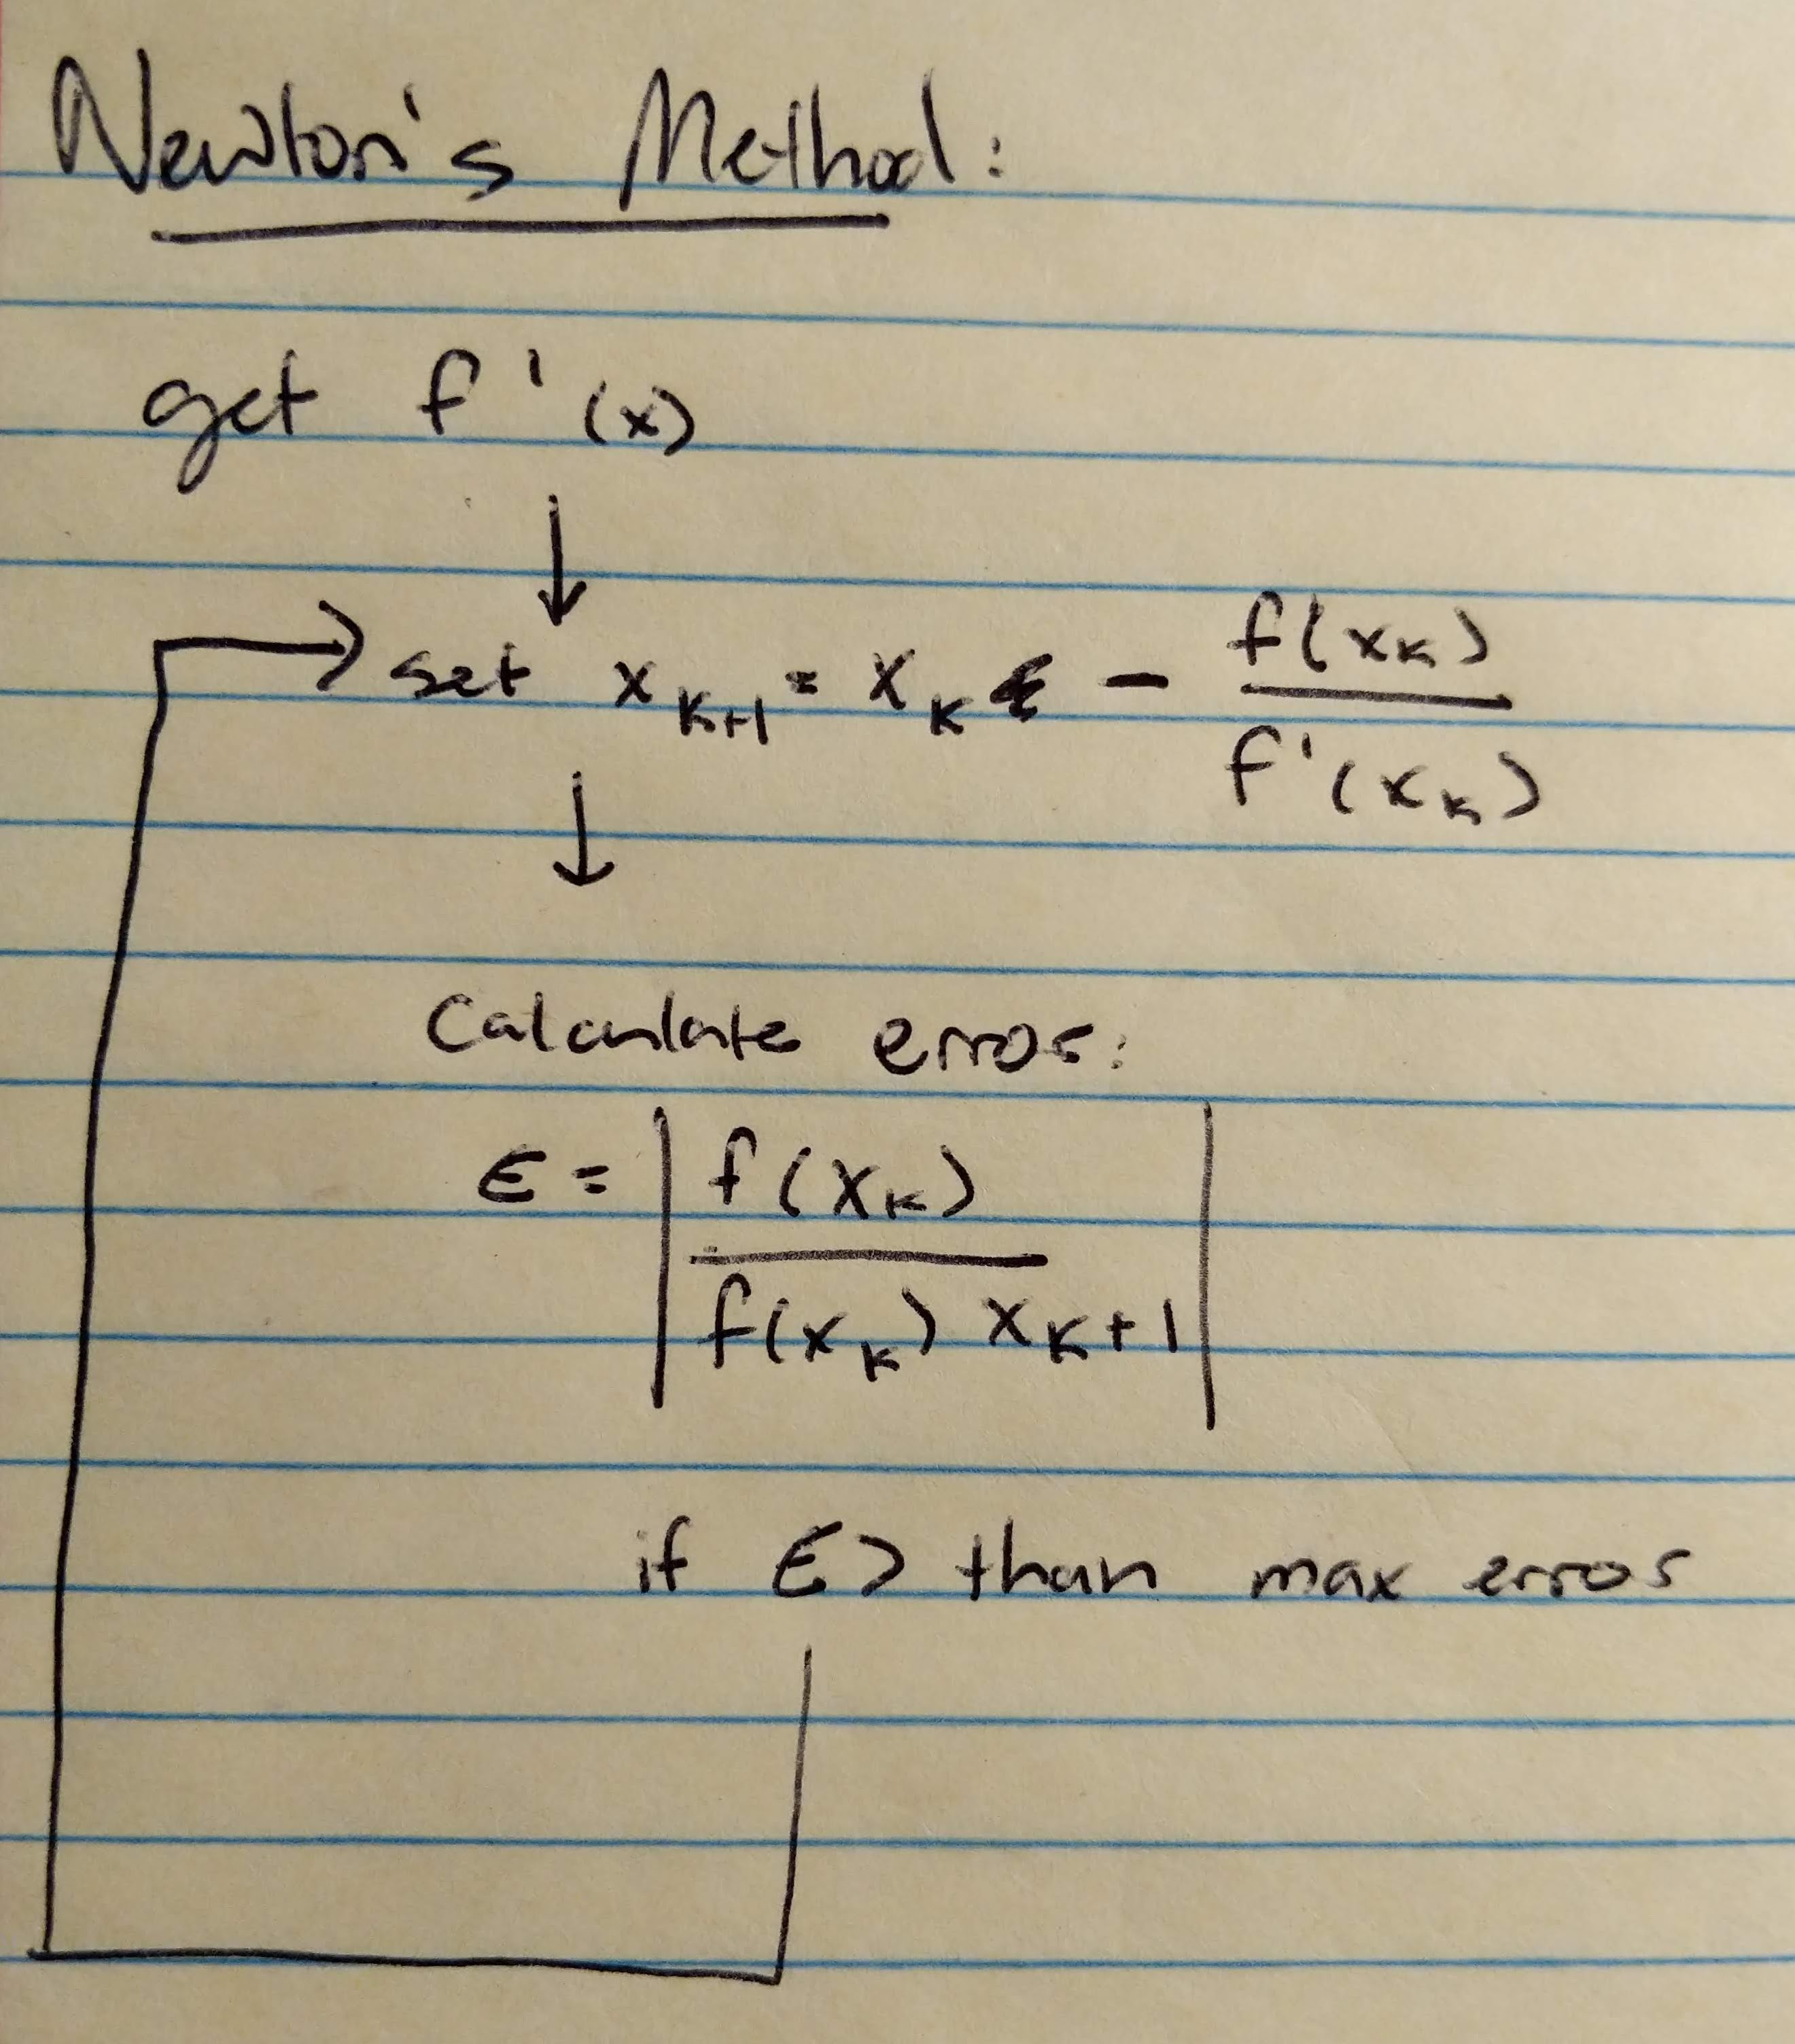
\includegraphics[width = .6\textwidth]{pic_4}
\end{center}
\item Here is a table showing iteration, $x_k$, and $\epsilon$ for the first root-finding problem.

\begin{center}
\begin{tabular}{|r|r|r|}
\hline
\multicolumn{1}{|l|}{Iteration:} & \multicolumn{1}{l|}{$x_k$} & \multicolumn{1}{l|}{$\epsilon$} \\ \hline
0 & 0.0001 & \multicolumn{1}{l|}{Inf} \\ \hline
1 & 12.1110599939339 & 0.999991743084416 \\ \hline
2 & 8.09254045425263 & 0.496570831174469 \\ \hline
3 & 5.41361087712689 & 0.494850782209803 \\ \hline
4 & 3.62778285976004 & 0.492264307540438 \\ \hline
5 & 2.43741808799465 & 0.488371189837504 \\ \hline
6 & 1.64412174520381 & 0.482504622972731 \\ \hline
7 & 1.11567626862556 & 0.473654850819105 \\ \hline
8 & 0.764004170068376 & 0.460301281504405 \\ \hline
9 & 0.530486635106756 & 0.4401949446184 \\ \hline
10 & 0.376190426783818 & 0.410154531687765 \\ \hline
11 & 0.275373819319325 & 0.366108178742967 \\ \hline
12 & 0.211187744354396 & 0.303928976376667 \\ \hline
13 & 0.172826641969727 & 0.221962898471344 \\ \hline
14 & 0.153391893645413 & 0.126699970007799 \\ \hline
15 & 0.147073149341482 & 0.042963275976772 \\ \hline
16 & 0.146368082588206 & 0.004817079931691 \\ \hline
17 & 0.146359505957651 & 5.86E-05 \\ \hline
\end{tabular}
\label{}
\end{center}

\newpage
\item Here is a table for the minimization problem, also showing iteration, $x_k$, and $\epsilon$. 
\begin{center}
\begin{tabular}{|r|r|r|}
\hline
\multicolumn{1}{|l|}{Iteration:} & \multicolumn{1}{l|}{$x_k$} & \multicolumn{1}{l|}{$\epsilon$} \\ \hline
0 & 0.0001 & \multicolumn{1}{l|}{Inf} \\ \hline
1 & 0.000149999999833 & 0.333333332592593 \\ \hline
2 & 0.000224999999188 & 0.333333331666667 \\ \hline
3 & 0.000337499996883 & 0.333333329583333 \\ \hline
4 & 0.000506249988917 & 0.333333324895831 \\ \hline
5 & 0.000759374961751 & 0.333333314348947 \\ \hline
6 & 0.001139062369644 & 0.333333290618432 \\ \hline
7 & 0.00170859330815 & 0.333333237224644 \\ \hline
8 & 0.002562889130906 & 0.333333117087963 \\ \hline
9 & 0.003844330890635 & 0.333332846777108 \\ \hline
10 & 0.005766486866465 & 0.333332238560854 \\ \hline
11 & 0.008649698338921 & 0.333330869989077 \\ \hline
12 & 0.012974439631194 & 0.333327790271208 \\ \hline
13 & 0.019461295288647 & 0.333320858721965 \\ \hline
14 & 0.029190713347596 & 0.333305251676902 \\ \hline
15 & 0.04378191598064 & 0.333270079808662 \\ \hline
16 & 0.065658822246247 & 0.333190659186057 \\ \hline
17 & 0.098440566721274 & 0.333010521646483 \\ \hline
18 & 0.147498131597946 & 0.332597873242183 \\ \hline
19 & 0.220683936420136 & 0.33163177170657 \\ \hline
20 & 0.329016592031842 & 0.329261983241325 \\ \hline
21 & 0.485904191232183 & 0.322877641377197 \\ \hline
22 & 0.696765770952346 & 0.302629073514841 \\ \hline
23 & 0.901552858583132 & 0.227149285459121 \\ \hline
24 & 0.948720416981045 & 0.049717026801222 \\ \hline
25 & 0.947747874126513 & 0.001026162000551 \\ \hline
26 & 0.947747133517416 & 7.81E-07 \\ \hline
\end{tabular}
\label{}
\end{center}
\end{enumerate}

\subsection{Comparison of Algorithms | Task List 1-C}
DO THIS!!!!


\section{Runge-Kutta Methods}


\end{document}